\section{Mining Similar Technology}
\label{sec:similarTech}

%We find comparable technologies by incorporating categorical information into word embedding of Stack Overflow tags.

Studies~\cite{barua2014developers, chen2016mining, treude2011programmers} show that Stack Overflow tags identify computer programming technologies that questions and answers revolve around. 
They cover a wide range of technologies, from algorithms (e.g.,  \textit{dijkstra, rsa}), programming languages (e.g., \textit{golang, javascript}), libraries and frameworks (e.g.,  \textit{gson, flask}), and development tools (e.g., \textit{sublime, vmware}). 
In this work, we regard Stack Overflow tags as a collection of technologies that developers would like to compare. 
We leverage word embedding techniques to infer semantically related tags, and develop natural language methods to analyze each tag's TagWiki to determine the corresponding technology's category (e.g., algorithm, library, IDE).
Finally, we build a knowledge base of comparable technologies by filtering the same-category, semantically-related tags. 

\subsection{Learning Tag Embeddings}
\label{sec:w2v}

\begin{figure}
	\centering
	\subfigure[Continuous skip-gram model]{%
		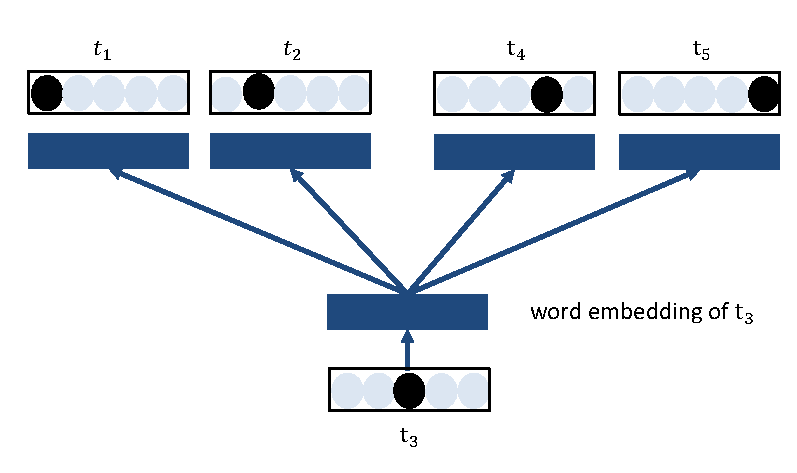
\includegraphics[width=0.23\textwidth]{figures/w2v_skip.pdf}
		\label{fig:w2v_skip}
	}
	\hfill
	\subfigure[Continuous bag-of-words model]{%
		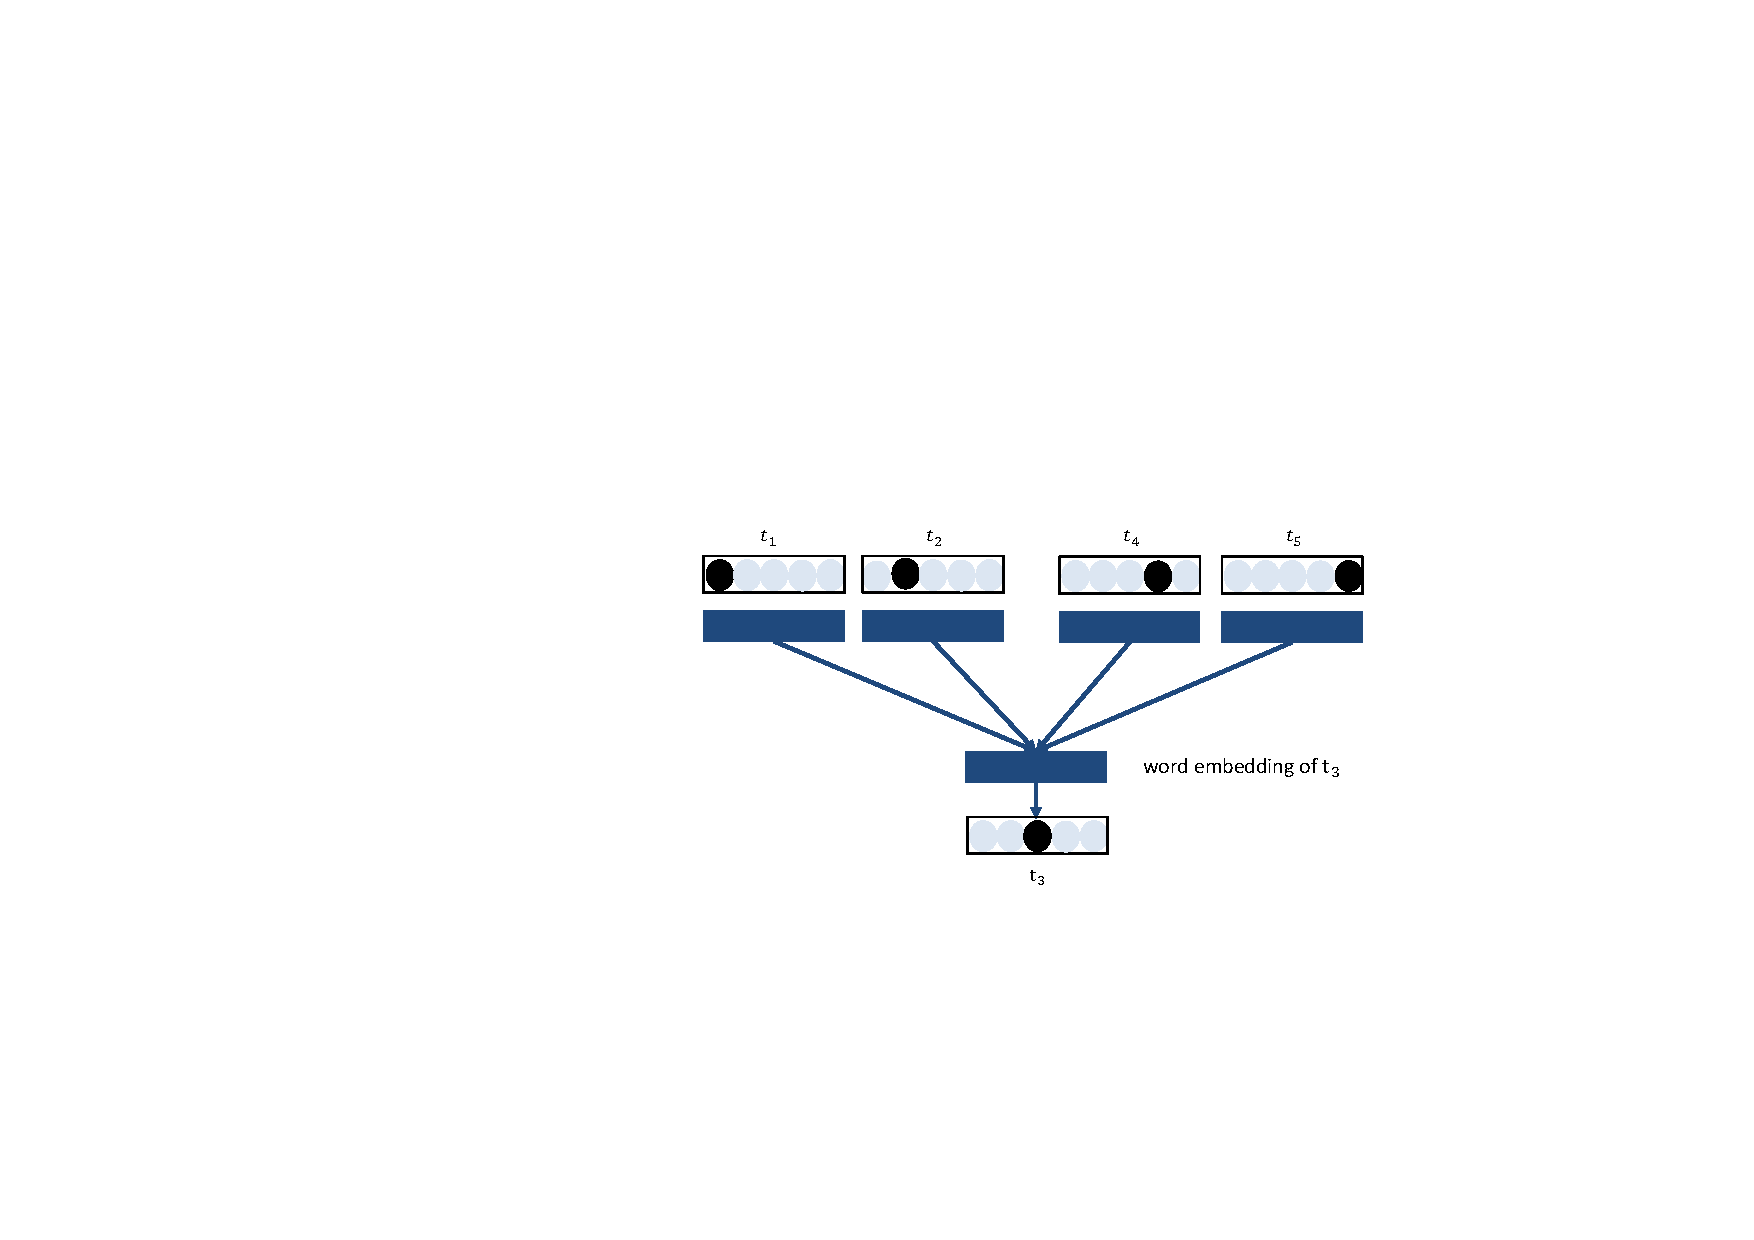
\includegraphics[width=0.23\textwidth]{figures/w2v_cbow.pdf}
		\label{fig:w2v_cbow}
	}
	\caption{The architecture of the two word embeddings models. The continuous skip-gram model predicts surrounding words given the central word, and the CBOW model predicts the central word based on the context words. Note the differences in arrow direction between the two models.
	}
	\vspace{-2mm}
	\label{fig:w2v}
\end{figure}

Word embeddings are dense low-dimensional vector representations of words that are built on the assumption that words with similar meanings tend to be present in similar context.
Studies~\cite{chen2016mining, mikolov2013efficient} show that word embeddings are able to capture rich semantic and syntactic properties of words for measuring word similarity.
In our approach, given a corpus of tag sentences, we use word embedding methods to learn the word representation of each tag using the surrounding context of the tag in the corpus of tag sentences.


There are two kinds of widely-used word embedding methods~\cite{mikolov2013efficient}, the continuous skip-gram model~\cite{mikolov2013distributed} and the continuous bag-of-words (CBOW) model.
As illustrated in Fig.~\ref{fig:w2v}, the objective of the continuous skip-gram model is to learn the word representation of each word that is good at predicting the co-occurring words in the same sentence (Fig.~\ref{fig:w2v_skip}), while the CBOW is the opposite, that is, predicting the center word by the context words (Fig.~\ref{fig:w2v_cbow}).
Note that word order within the context window is not important for learning word embeddings.

Specifically, given a sequence of training text stream $t_{1}, t_{2}, ..., t_{k}$, the objective of the continuous skip-gram model is to maximize the following average log probability:
\begin{equation}
L = \frac{1}{K}\sum_{k=1}^{K} \sum_{-N\preceq j \preceq N, j\neq0} \log p(t_{k+j}|t_{k})
\label{equ:condition_skip}
\end{equation}
while the objective of the CBOW model is:
\begin{equation}
L = \frac{1}{K}\sum_{k=1}^{K} \log p(t_{k}|(t_{k-N}, t_{k-N+1}, ..., t_{k+N}) )
\label{equ:condition_cbow}
\end{equation}
where $t_{k}$ is the central word, $t_{k+j}$ is its surrounding word with the distance $j$, and $N$ indicates the window size.
In our application of the word embedding, a tag sentence is a training text stream, and each tag is a word.
As tag sentence is short (has at most 5 tags), we set $N$ as 5 in our approach so that the context of one tag is all other tags in the current sentences.
That is, the context window contains all other tags as the surrounding words for a given tag.
Therefore, tag order does not matter in this work for learning tag embeddings.

\begin{comment}
The probability $p(t_{k+j}|t_{k})$  or $p(t_{k}|(t_{k-j}, t_{k-j+1}, ..., t_{k+j}) )$ in Eq.~\ref{equ:condition_skip} and Eq.~\ref{equ:condition_cbow} can be formulated as a log-linear softmax function which can be efficiently solved by the negative sampling method~\cite{mikolov2013distributed}.
After the iterative feed-forward and back propagation, the training process finally converges, and each tag obtains a low-dimension vector as its word representation (i.e., tag embedding) in the resulting vector space.	
\end{comment}
To determine which word-embedding model performs better in our comparable technology reasoning task , we carry out a comparison experiment, and the details are discussed in Section~\ref{sec:comparison_w2v}.



\subsection{Mining Categorical Knowledge}

\label{sec:categoryKG}

\begin{comment}
\begin{figure}
	\centering
	\begin{tikzpicture}
	%\tikzset{level distance=1cm}
	%\tikzset{sibling distance=0.3cm}
	\tikzstyle{level 1}=[level distance=0.8cm, sibling distance=0.1cm]
	\tikzstyle{level 2}=[level distance=0.8cm, sibling distance=0.1cm]
	\tikzstyle{level 3}=[level distance=0.8cm, sibling distance=0.1cm]
	\tikzstyle{every node}=[font=\scriptsize]
	
	\Tree [.S [.NP [.NNS iOS ] ]
	[.VBZ is ]
	[.DT a ]
	[.JJ mobile ]
	[.NP [.NN operating ] [.NN system ] ]
	[.VBD developed ]
	[.IN by ]
	[.NP [.NNP Apple ] ]
	]
	
	\end{tikzpicture}
	\caption{POS tagging and phrase chunking results of the definition sentence of the tag \textit{iOS} \textcolor{red}{Change this example}}
	\label{fig:exampleChunking}
\end{figure}	
\end{comment}

\begin{figure}
	\centering
	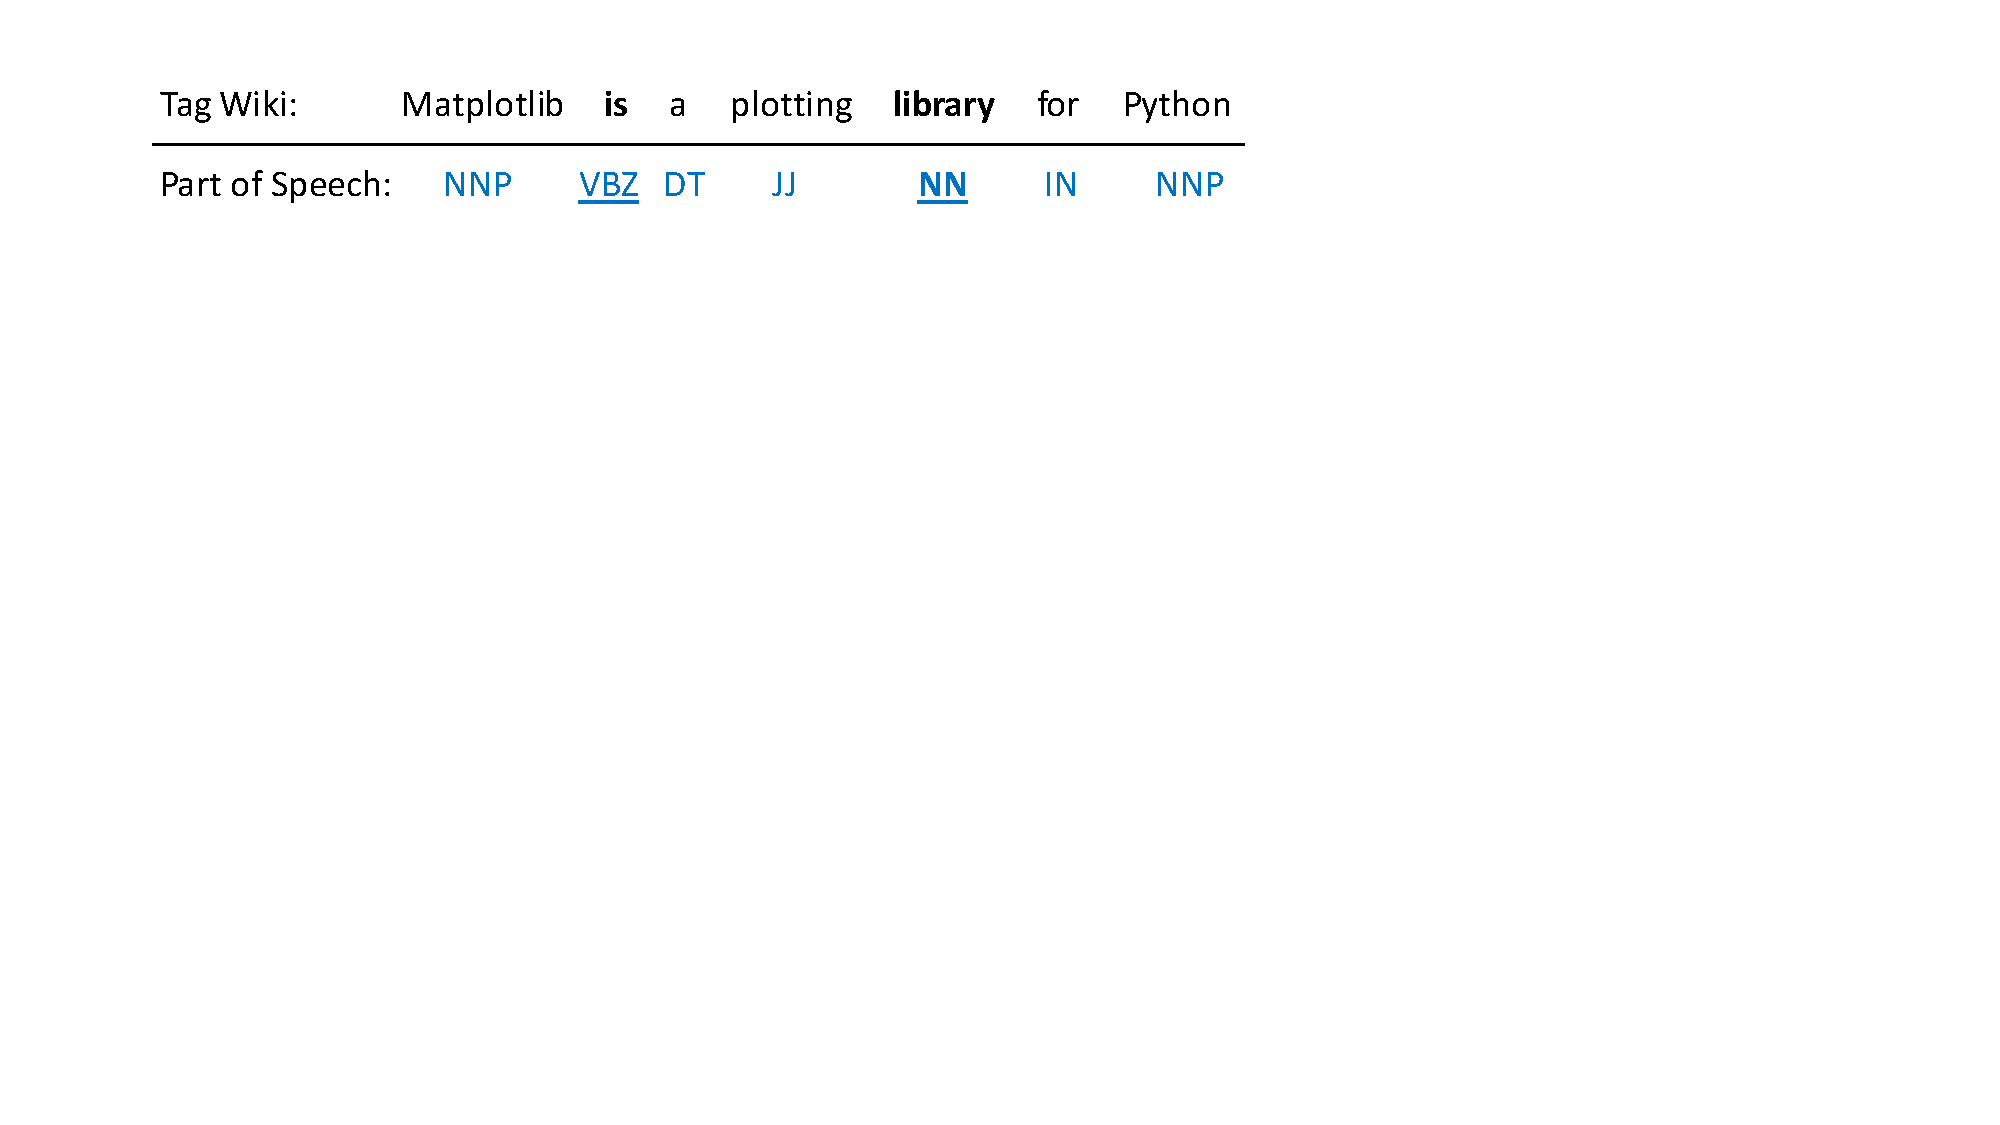
\includegraphics[width=0.46\textwidth]{figures/pos.pdf}
	\vspace{-3mm}
	\caption{POS tagging of the definition sentence of the tag \textit{RSA}}
	\vspace{-2mm}
	\label{fig:exampleChunking}
\end{figure}
In Stack Overflow, tags can be of different categories, such as programming language, library, framework, tool, API, algorithm, etc.
To determine the category of a tag, we resort to the tag definition in the TagWiki of the tag.
The TagWiki of a tag is collaboratively edited by the Stack Overflow community.
Although there are no strict formatting rules in Stack Overflow, the TagWiki description usually starts with a short sentence to define the tag.
For example, the tagWiki of the tag \textit{Matplotlib} starts with the sentence ``Matplotlib is a plotting library for Python''.
Typically, the first noun just after the \textit{be} verb defines the category of the tag.
For example, from the tag definition of \textit{Matplotlib}, we can learn that the category of \textit{Matplotlib} is \textit{library}.

Based on the above observation of tag definitions, we use the NLP methods~\cite{kazama2007exploiting, chen2016mining} to extract such noun from the tag definition sentence as the category of a tag.
%The overview of extracting categorical knowledge can be seen in Figure.\ref{fig:flowChartCategory}.
Given the tagWiki of a tag in Stack Overflow, we extract the first sentence of the TagWiki description, and clean up the sentence by removing hyperlinks and brackets such as ``\{\}'', ``()''.
Then, we apply Part of Speech (POS) tagging to the extracted sentence.
POS tagging is the process of marking up a word in a text as corresponding to a particular part of speech, such as noun, verb, adjective.
%Phrase chunking is the process of segmenting a sentence into its subconstituents, such as noun phrases, verb phrases.
NLP tools usually agree on the POS tags of nouns, and we find that POS tagger in NLTK~\cite{bird2004nltk} is especially suitable for our task.
In NLTK, the noun is annotated by different POS tags~\cite{web:nltktag} including NN (Noun, singular or mass), NNS (Noun, plural), NNP (Proper noun, singular), NNPS (Proper noun, plural).
%Then we use the phrase chunking i.e., regular expression to recognize consecutive nouns (at least one noun) as noun phrase by their POS tags.
%We adopt the default POS tagging and \textcolor{red}{??phrase chunking} implemented in NLTK\footnote{\url{http://www.nltk.org/_modules/nltk/tag.html}}.
%NLTK supports POS tags defined in the Penn Treebank Project\footnote{\url{https://www.ling.upenn.edu/courses/Fall_2003/ling001/penn_treebank_pos.html}}.
Fig.~\ref{fig:exampleChunking} shows the results for the tag definition sentence of \textit{RSA}.
Based on the POS tagging results, we extract the first noun  (\textit{algorithm} in this example) after the be verb (\textit{is} in this example) as the category of the tag.
That is, the category of \textit{RSA} is \textit{algorithm}.
Note that if the noun is some specific words such as \textit{system}, \textit{development}, we will further check its neighborhood words to see if it is \textit{operating system} or \textit{independent development environment}.

With this method, we obtain 318 categories for the 23,658 tags (about 67\% of all the tags that have TagWiki).
We manually normalize these 318 categories labels, such as merging \textit{app} and \textit{applications} as \textit{application}, \textit{libraries} and \textit{lib} as \textit{library}, and normalizing uppercase and lowercase (e.g., \textit{API} and \textit{api}).
As a result, we obtain 167 categories.
Furthermore, we manually categorize these 167 categories into five general categories: programming language, platform, library, API, and concept/standard~\cite{ye2016software}.
This is because the meaning of the fine-grained categories is often overlapping, and there is no consistent rule for the usage of these terms in the TagWiki.
This generalization step is necessary, especially for the library tags that broadly refer to the tags whose fine-grained categories can be library, framework, api, toolkit, wrapper, and so on.
%\footnote{A complete list can be found at \url{https://graphofknowledge.appspot.com/libCategory}}
For example, in Stack Overflow's TagWiki, \textit{junit} is defined as a framework, \textit{google-visualization} is defined as an API, and \textit{wxpython} is defined as a wrapper. 
All these tags are referred to as library tags in our approach.


Although the above method obtains the tag category for the majority of the tags, the first sentence of the TagWiki of some tags is not formatted in the standard ``tag be noun phrase'' form.
For example, the first sentence of the TagWiki of the tag \textit{itext} is ``Library to create and manipulate PDF documents in Java'', or for \textit{markermanager}, the tag definition sentence is ``A Google Maps tool'', or for \textit{ghc-pkg}, the tag definition sentence is ``The command ghc-pkg can be used to handle GHC packages''.
As there is no \textit{be} verb in this sentence, the above NLP method cannot return a noun phrase as the tag category.
According to our observation, for most of such cases, the category of the tag is still present in the sentence, but often in many different ways.
It is very likely that the category word appears as the first noun phrase that match the existing category words in the definition sentence.
Therefore, we use a dictionary look-up method to determine the category of such tags.
Specially, we use the 167 categories obtained using the above NLP method as a dictionary to recognize the category of the tags that have not been categorized using the NLP method.
Given an uncategorized tag, we scan the first sentence of the tag's TagWiki from the beginning, and search for the first match of a category label in the sentence.
If a match is found, the tag is categorized as the matched category.
For example, the tag \textit{itext} is categorized as \textit{library} using this dictionary look-up method.
Using the dictionary look-up method, we obtain the category for 9,648 more tags.

Note that we cannot categorize some (less than 15\%) of the tags using the above NLP method and the dictionary look-up method.
This is because these tags do not have a clear tag definition sentence, for example, the TagWiki of the tag \textit{richtextbox} states that ``The RichTextBox control enables you to display or edit RTF content''.
This sentence is not a clear definition of what \textit{richtextbox} is.
Or no category match can be found in the tag definition sentence of some tags.
For example, the TagWiki of the tag \textit{carousel} states that ``A rotating display of content that can house a variety of content''.
Unfortunately, we do not have the category ``display'' in the 167 categories we collect using the NLP method.
When building comparable-technologies knowledge base, we exclude these uncategorized tags as potential candidates.

\subsection{Building Similar-technology Knowledge Base}
Given a technology tag $t_1$ with its vector $vec(t_1)$, we first find most similar library $t_2$ whose vector $vec(t_2)$ is most closed to it, i.e.,
\begin{equation}
	\operatornamewithlimits{argmax}_{t_2 \in T}  \cos (vec(t_1), vec(t_2)) 
	\label{equ:similarity}
\end{equation} 
where $T$ is the set of technology tags excluding $t_1$, and $cos(u, v)$ is the cosine similarity of the two vectors.

\begin{table}
	\small
	\center	
	\caption{Examples of filtering results by categorical knowledge (in red)}
	\vspace{-2mm}
	\setlength{\tabcolsep}{0.2em}
	\begin{tabular}{l|l}
		\hline
		\textbf{Source} & \textbf{Top-5 recommendations from word embedding} \\
		\hline
		nltk   & \textcolor{red}{\st{nlp}}, opennlp, gate, \textcolor{red}{\st{language-model}}, stanford-nlp \\
		tcp    & tcp-ip, \textcolor{red}{\st{network-programming}}, udp, \textcolor{red}{\st{packets}}, \textcolor{red}{\st{tcpserver}} \\
		vim    & sublimetext, \textcolor{red}{\st{vim-plugin}}, emacs, nano, gedit\\
		swift  & objective-c, \textcolor{red}{\st{cocoa-touch}}, \textcolor{red}{\st{storyboard}}, \textcolor{red}{\st{launch-screen}} \\%,\textcolor{red}{\st{asset-catalog}} \\
		%unicode & gbk, utf, 
		bubble-sort & insertion-sort, selection-sort, mergesort, timsort, heapsort \\
				\hline
	\end{tabular}
	\vspace{-3mm}
	\label{tab:filterResult}
\end{table}

Note that tags whose tag embedding is similar to the vector $vec(t_1)$ may not always be in the same category.
For example, tag embeddings of the tags \textit{nlp}, \textit{language-model} are similar to the vector $vec(nltk)$.
These tags are relevant to the \textit{nltk} library as they refer to some NLP concepts and tasks, but they are not comparable libraries to the \textit{nltk}.
In our approach, we rely on the category of tags (i.e., categorical knowledge) to return only tags within the same category as candidates.
Some examples can be seen in Table~\ref{tab:filterResult}.


In practice, there could be several comparable technologies $t_2$ to the technology $t_1$.
Thus, we select tags $t_2$ with the cosine similarity in Eq.~\ref{equ:similarity} above a threshold $Thresh$.
Take the library \textit{nltk} (a NLP library in python) as an example.
We will preserve several candidates which are libraries such as \textit{textblob}, \textit{stanford-nlp}.